\documentclass[tikz, border=12pt]{standalone}
\usepackage{tikz}
\usepackage{amsmath}
\usetikzlibrary{arrows.meta, calc}

\definecolor{mfill}{RGB}{210,225,245}
\definecolor{mline}{RGB}{ 50, 80,140}
\definecolor{cfill}{RGB}{255,240,200}
\definecolor{cline}{RGB}{160,110,  0}
\definecolor{dcol} {RGB}{140,  0,  0}
\definecolor{acol} {RGB}{ 20,120, 20}

\tikzset{
  ME/.style={draw=mline, line width=0.9pt},
  CE/.style={draw=cline, line width=1.1pt},
  DA/.style={dcol,{Latex[length=3.5pt]}-{Latex[length=3.5pt]},line width=0.65pt},
  DE/.style={dcol, line width=0.5pt},
  AX/.style={acol, line width=0.6pt,
             dash pattern=on 5pt off 2pt on 1.5pt off 2pt},
}

\newcommand{\PX}{0.32}
\newcommand{\PY}{0.18}

\begin{document}
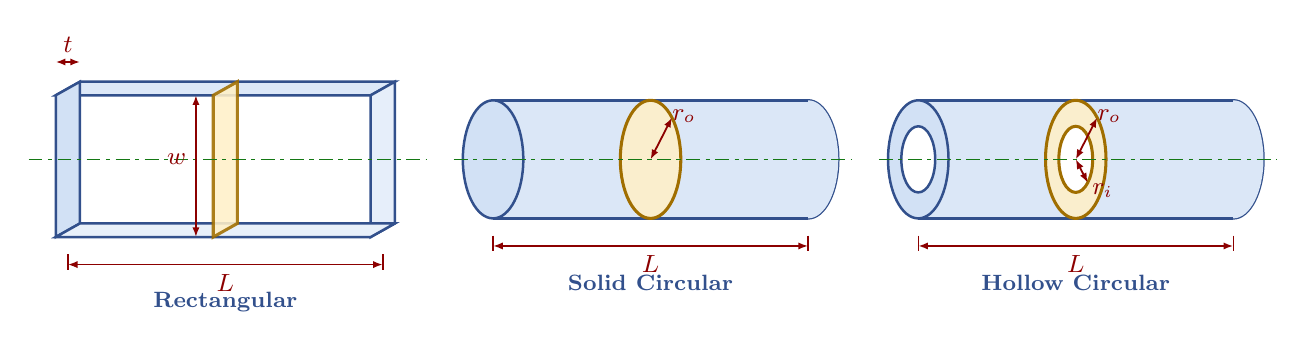
\begin{tikzpicture}

%% ================================================================
%%  MEMBER 1 – RECTANGULAR
%% ================================================================
\begin{scope}[xshift=0cm]
  \pgfmathsetmacro{\W}{0.9}
  \pgfmathsetmacro{\T}{0.48}
  \pgfmathsetmacro{\LL}{4.0}
  \pgfmathsetmacro{\dx}{\T*\PX}
  \pgfmathsetmacro{\dy}{\T*\PY}

  % top face
  \fill[mfill!75, ME]
    (-\dx,\W-\dy) -- (\LL-\dx,\W-\dy) -- (\LL+\dx,\W+\dy) -- (\dx,\W+\dy) -- cycle;
  % right face
  \fill[mfill!55, ME]
    (\LL+\dx,\W+\dy) -- (\LL+\dx,-\W+\dy) -- (\LL-\dx,-\W-\dy) -- (\LL-\dx,\W-\dy) -- cycle;
  % front face
  \fill[mfill, ME]
    (-\dx,-\W-\dy) -- (-\dx,\W-\dy) -- (\dx,\W+\dy) -- (\dx,-\W+\dy) -- cycle;
  % bottom face
  \fill[mfill!50, ME]
    (-\dx,-\W-\dy) -- (\LL-\dx,-\W-\dy) -- (\LL+\dx,-\W+\dy) -- (\dx,-\W+\dy) -- cycle;

  % cut plane at midspan
  \pgfmathsetmacro{\mx}{\LL/2}
  \fill[cfill, CE, opacity=0.88]
    (\mx-\dx,-\W-\dy) -- (\mx-\dx,\W-\dy) -- (\mx+\dx,\W+\dy) -- (\mx+\dx,-\W+\dy) -- cycle;

  % longitudinal axis
  \draw[AX] (-0.5,0) -- (\LL+0.55,0);

  % dim w
  \draw[DA] (\mx-\dx-0.22,-\W-\dy) -- (\mx-\dx-0.22,\W-\dy);
  \node[dcol, left, font=\small] at (\mx-\dx-0.22,0) {$w$};

  % dim t
  \draw[DA] (-\dx,\W+\dy+0.25) -- (\dx,\W+\dy+0.25);
  \node[dcol, above, font=\small] at (0,\W+\dy+0.25) {$t$};

  % dim L
  \pgfmathsetmacro{\ybot}{-\W-\dy}
  \draw[DE] (0,\ybot-0.22) -- (0,\ybot-0.42);
  \draw[DE] (\LL,\ybot-0.22) -- (\LL,\ybot-0.42);
  \draw[DA] (0,\ybot-0.35) -- (\LL,\ybot-0.35);
  \node[dcol, below, font=\small] at (\LL/2,\ybot-0.35) {$L$};

  \node[mline, font=\footnotesize\bfseries] at (\LL/2,\ybot-0.82) {Rectangular};
\end{scope}

%% ================================================================
%%  MEMBER 2 – SOLID CIRCULAR
%% ================================================================
\begin{scope}[xshift=5.4cm]
  \pgfmathsetmacro{\R}{0.75}
  \pgfmathsetmacro{\LL}{4.0}
  \pgfmathsetmacro{\ex}{\R*\PX*1.6}

  % back ellipse
  \fill[mfill!60] (\LL,0) ellipse [x radius=\ex, y radius=\R];
  \draw[ME]       (\LL,0) ellipse [x radius=\ex, y radius=\R];

  % body fill between ellipses
  \fill[mfill!80]
    (0,\R) -- (\LL,\R)
    arc[start angle=90, end angle=-90, x radius=\ex, y radius=\R]
    -- (0,-\R)
    arc[start angle=-90, end angle=90, x radius=\ex, y radius=\R]
    -- cycle;

  \draw[mline, line width=0.9pt] (0,\R) -- (\LL,\R);
  \draw[mline, line width=0.9pt] (0,-\R) -- (\LL,-\R);

  % front ellipse
  \fill[mfill] (0,0) ellipse [x radius=\ex, y radius=\R];
  \draw[ME]    (0,0) ellipse [x radius=\ex, y radius=\R];

  % cut ellipse
  \pgfmathsetmacro{\mx}{\LL/2}
  \fill[cfill, opacity=0.88] (\mx,0) ellipse [x radius=\ex, y radius=\R];
  \draw[CE]                   (\mx,0) ellipse [x radius=\ex, y radius=\R];

  % axis
  \draw[AX] (-0.5,0) -- (\LL+0.55,0);

  % dim r_o
  \draw[DA] (\mx,0) -- ++(\ex*0.707,\R*0.707);
  \node[dcol, above right, font=\small] at (\mx+\ex*0.4,\R*0.45) {$r_o$};

  % dim L
  \draw[DE] (0,-\R-0.22) -- (0,-\R-0.42);
  \draw[DE] (\LL,-\R-0.22) -- (\LL,-\R-0.42);
  \draw[DA] (0,-\R-0.35) -- (\LL,-\R-0.35);
  \node[dcol, below, font=\small] at (\LL/2,-\R-0.35) {$L$};

  \node[mline, font=\footnotesize\bfseries] at (\LL/2,-\R-0.82) {Solid Circular};
\end{scope}

%% ================================================================
%%  MEMBER 3 – HOLLOW CIRCULAR
%% ================================================================
\begin{scope}[xshift=10.8cm]
  \pgfmathsetmacro{\Ro}{0.75}
  \pgfmathsetmacro{\Ri}{0.42}
  \pgfmathsetmacro{\LL}{4.0}
  \pgfmathsetmacro{\exo}{\Ro*\PX*1.6}
  \pgfmathsetmacro{\exi}{\Ri*\PX*1.6}

  % back outer ellipse
  \fill[mfill!60] (\LL,0) ellipse [x radius=\exo, y radius=\Ro];
  \draw[ME]       (\LL,0) ellipse [x radius=\exo, y radius=\Ro];
  \fill[white]    (\LL,0) ellipse [x radius=\exi, y radius=\Ri];
  \draw[ME]       (\LL,0) ellipse [x radius=\exi, y radius=\Ri];

  % body
  \fill[mfill!80]
    (0,\Ro) -- (\LL,\Ro)
    arc[start angle=90, end angle=-90, x radius=\exo, y radius=\Ro]
    -- (0,-\Ro)
    arc[start angle=-90, end angle=90, x radius=\exo, y radius=\Ro]
    -- cycle;

  \draw[mline, line width=0.9pt] (0,\Ro)  -- (\LL,\Ro);
  \draw[mline, line width=0.9pt] (0,-\Ro) -- (\LL,-\Ro);

  % front outer ellipse
  \fill[mfill] (0,0) ellipse [x radius=\exo, y radius=\Ro];
  \draw[ME]    (0,0) ellipse [x radius=\exo, y radius=\Ro];
  \fill[white] (0,0) ellipse [x radius=\exi, y radius=\Ri];
  \draw[ME]    (0,0) ellipse [x radius=\exi, y radius=\Ri];

  % cut annular face
  \pgfmathsetmacro{\mx}{\LL/2}
  \fill[cfill, opacity=0.88] (\mx,0) ellipse [x radius=\exo, y radius=\Ro];
  \fill[white]               (\mx,0) ellipse [x radius=\exi, y radius=\Ri];
  \draw[CE] (\mx,0) ellipse [x radius=\exo, y radius=\Ro];
  \draw[CE] (\mx,0) ellipse [x radius=\exi, y radius=\Ri];

  % axis
  \draw[AX] (-0.5,0) -- (\LL+0.55,0);

  % dim r_o
  \draw[DA] (\mx,0) -- ++(\exo*0.707,\Ro*0.707);
  \node[dcol, above right, font=\small] at (\mx+\exo*0.4,\Ro*0.45) {$r_o$};

  % dim r_i
  \draw[DA] (\mx,0) -- ++(\exi*0.707,-\Ri*0.707);
  \node[dcol, below right, font=\small] at (\mx+\exi*0.4,-\Ri*0.45) {$r_i$};

  % dim L
  \draw[DE] (0,-\Ro-0.22) -- (0,-\Ro-0.42);
  \draw[DE] (\LL,-\Ro-0.22) -- (\LL,-\Ro-0.42);
  \draw[DA] (0,-\Ro-0.35) -- (\LL,-\Ro-0.35);
  \node[dcol, below, font=\small] at (\LL/2,-\Ro-0.35) {$L$};

  \node[mline, font=\footnotesize\bfseries] at (\LL/2,-\Ro-0.82) {Hollow Circular};
\end{scope}

\end{tikzpicture}
\end{document}
